\documentclass[2pt]{amsart}

\usepackage[english]{babel}
\usepackage {amsmath} 
\usepackage{amssymb}
\usepackage{amsfonts}
\usepackage{amsthm}
\usepackage{graphicx}
\usepackage[colorlinks,linkcolor=blue, citecolor=blue,urlcolor=blue]{hyperref}
\usepackage[backend=bibtex]{biblatex}

%% Environments for theorems, etc.. 
\theoremstyle{theorem} % set the style for the following theorems
\newtheorem{thm}{Theorem}[section] %\newtheorem{name}{display-text}[numbered-within]
\newtheorem{lem}[thm]{Lemma} %\newtheorem{name}[numbered-like]{display-text}
\newtheorem{cor}[thm]{Corollary}
\newtheorem{prop}[thm]{Proposition}
\newtheorem{alg}[thm]{Algorithm}
\theoremstyle{definition}       
\newtheorem{defn}[thm]{Definition}
\newtheorem{conj}[thm]{Conjecture}
\theoremstyle{example}                     
\newtheorem{prob}[thm]{Problem}
\theoremstyle{remark}                       
\newtheorem{exmp}[thm]{Example}
\newtheorem{rem}[thm]{Remark}
\newtheorem{claim}[thm]{Claim}  
\renewcommand{\theclaim}{}

\numberwithin{equation}{section}

\newcommand{\R}{\mathbb{R}}
\newcommand{\Q}{\mathbb{Q}}
\newcommand{\N}{\mathbb{N}}
\newcommand{\Z}{\mathbb{Z}}
\DeclareMathOperator{\rank}{rank}
\DeclareMathOperator{\dimension}{dim}
\DeclareMathOperator*{\supp}{supp}

\addbibresource{wavelet.bib}


\author{Jason Ngo}
\begin{document}
	
\section{Introduction}
Since the start of the 20th century, we have seen rapid development in the theory and applications of wavelets. As a mathematical tool, wavelets can be used to extract information from different kinds of data such as audio signals and images.

This paper will explore what wavelets are; introduce readers to the first orthonormal wavelet basis, the Haar system; approximate functions using Haar wavelets; and discuss their applications in image compression.

\section{Definitions}
This section is based on paper [???].

\begin{defn} \label{def:l2}
	\emph{$ L^2(\R) $ space} is the set of all functions $ f: \R \to \R $ such that the integral of $ f^2 $ over the whole real line is finite, taken with the norm
	\[ \|f\|_2^2 = \int_{-\infty}^{\infty} |f(x)|^2 dx. \]
\end{defn}

\underline{Consider changing the notation to $ \int_\R $ instead.}

\begin{defn} \label{def:orthonormal}
	A set of functions $ \{\ \varphi \}_{k=1}^N $ is said to be an \emph{orthonormal basis} for the N-dimensional space $ V $ if:
	\begin{enumerate}
		\item Every $ u \in V $ can be written as $ u = \sum_{k=1}^N c_k \varphi_k $ for some scalar $ c_k $\footnote{We can easily prove that $ c_k = \langle u,\varphi_k \rangle $, for $ k = 1,2,\cdots,N. $}.
		\item $ \langle \varphi_j, \varphi_k \rangle = 0 $ if $ j \neq k $.
		\item $ \langle \varphi_j, \varphi_k \rangle = 1 $ if $ j = k $.
	\end{enumerate}
\end{defn}

\begin{defn} \label{def:support}
	The \emph{support} of a real-valued function $ f $ is the subset of the domain containing those elements which are are not mapped to zero.
	
	Example: The \emph{support} of the Haar wavelet is $ [0,1] $.
	Notation: $ \supp \varPsi = [0,1] $.
\end{defn}

\begin{defn} \label{def: wavelet}
	A \emph{wavelet} is a function $ \varPsi \in L^2(\R) $ such that the set
	\[ \{ \varPsi_{j,k}(x) = 2^{j/2} \varPsi (2^j x-k): j,k \in \Z  \} \]
	forms an orthonormal basis for $ L^2(\R) $. Sometimes $ \varPsi $ is called the \emph{mother wavelet}.
\end{defn}

Observe that all $ \varPsi_{j,k} $ are generated by shifting and scaling\footnote{The dilations here are taken to be powers of 2.} the wavelet $ \varPsi $ and that each $ \varPsi_{j,k} $ is normalized so that $ \| \varPsi_{j,k}\|_2 = \|\varPsi\|_2 = 1 $ for all $ j,k \in \Z $.

Now, let us explore one particular type of wavelet that has many applications in noise filtering and image processing: \emph{The Haar Wavelet}.

\begin{quote}
	The child wavelets $ \varPsi_{j,k} $ are simply dilated and translated versions of the mother wavelet multiplied with the normalization factor 2j/2. The normalization factor is there so that the dilated and translated Haar function satisfies property (2) in the wavelet	definition.
\end{quote}

\begin{defn}
	The \emph{Haar wavelet} is the function $ \varPsi = \chi_{[0,0.5)} - \chi_{[0.5,1)} $, where $ \chi $ is the characteristic function. The \emph{Haar wavelet basis is the family $ \{ \varPsi_{j,k}:j,k \in \Z \} $}.
\end{defn}
See Figure \ref{fig:haarsystem} for examples of some elements of the Haar wavelet basis, obtained by translating and/or stretching the Haar wavelet. 

\begin{figure}
	\centering
	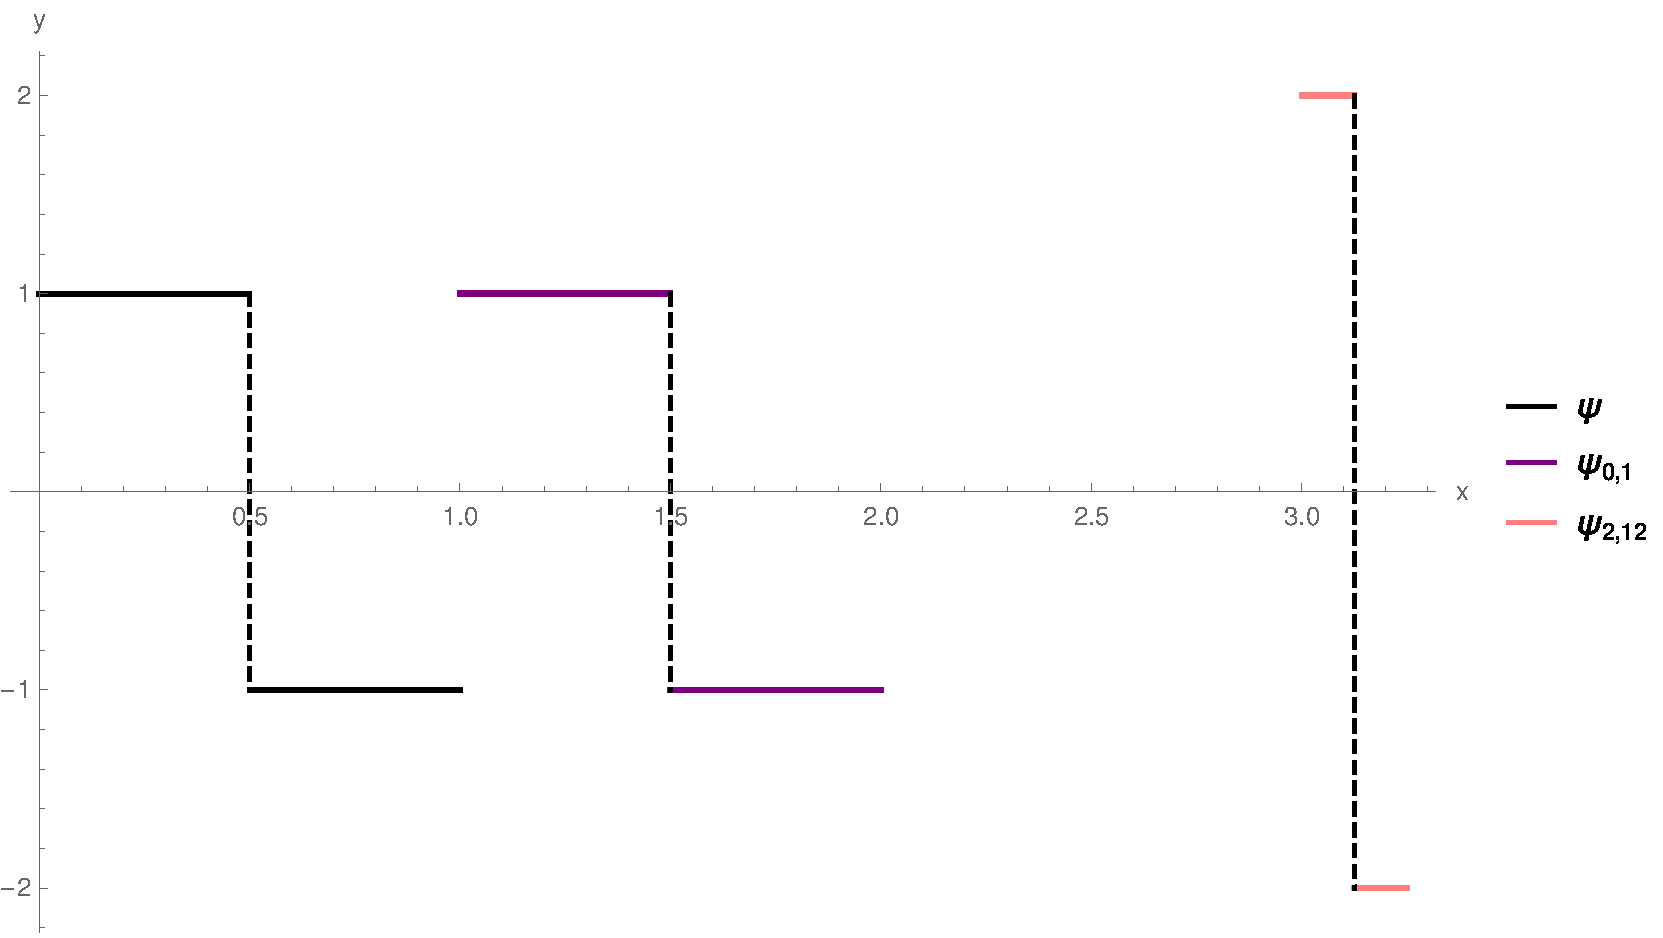
\includegraphics[width=0.7\linewidth]{img/haar_system}
	\caption[Elements of the Haar system]{Elements of the Haar system: $ \varPsi, \varPsi_{0,1} $ and $ \varPsi_{2,12} $}
	\label{fig:haarsystem}
\end{figure}

Note that $ \varPsi_{j,k} $ has width of order $ 2^{-j} $, and is centered about $ k 2^{-j} $. We can see that the Haar wavelet $ \varPsi $ has the following properties:
\begin{enumerate}
	\item $ \int_{-\infty}^{\infty} \varPsi(x)dx = 0 $, which makes it a wave.
	\item  $ \int_{-\infty}^{\infty} \varPsi(x)^2dx = 1 $, i.e. the norm is 1.
\end{enumerate}

Now, our task is to prove that the Haar wavelet is in fact a wavelet, i.e. the Haar wavelet basis is an orthonormal basis for $ L^2(\R) $.

	
\end{document}